% Editable native annotations around unchanged verified IDE photographs.
\par
\begin{figure}[htbp]
\centering
\newsavebox{\MARSppmsaveregistersBox}
\sbox{\MARSppmsaveregistersBox}{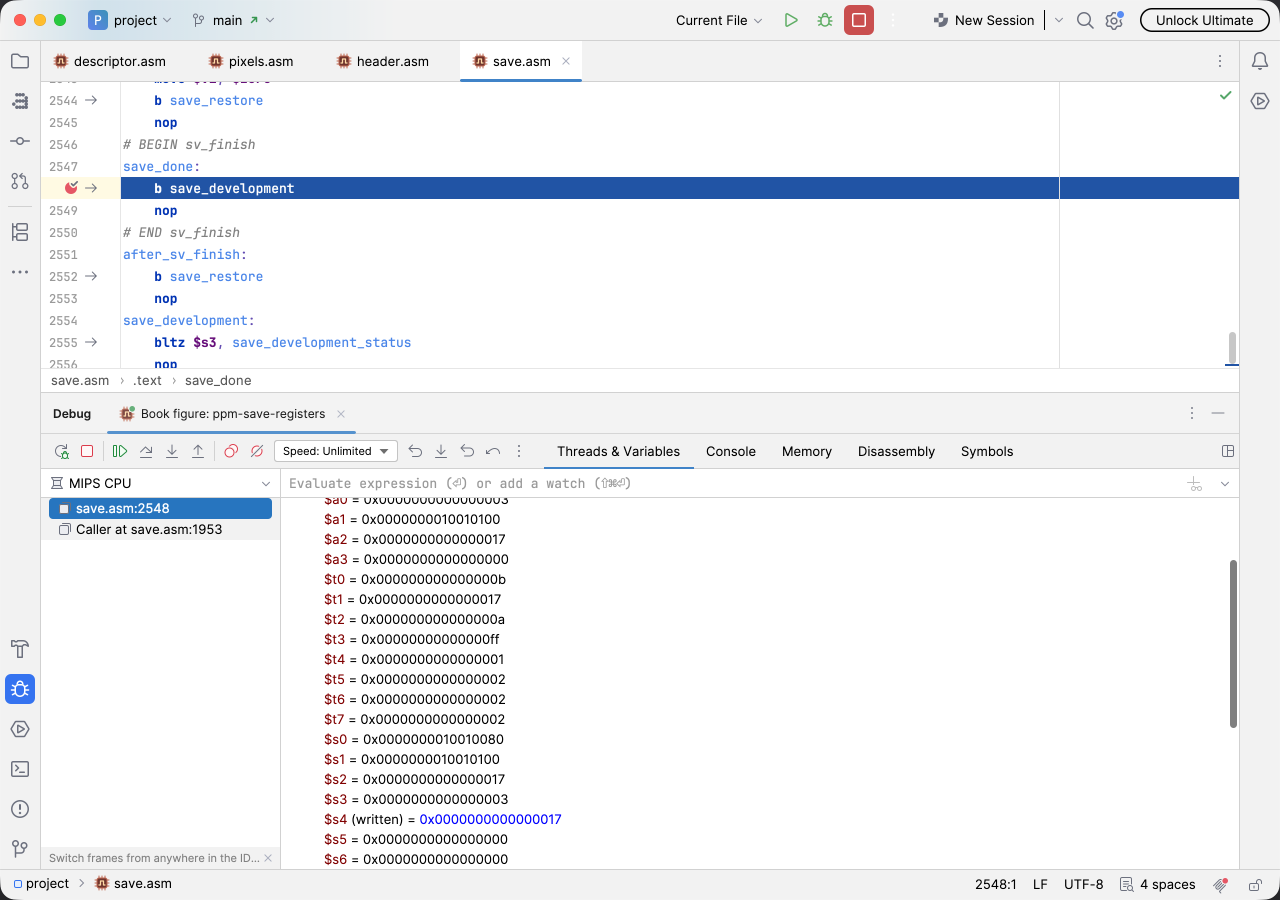
\includegraphics[artifact]{packages/029-binary-ppm/captures/f04/registers.png}}
\newsavebox{\MARSppmsavesourceBox}
\sbox{\MARSppmsavesourceBox}{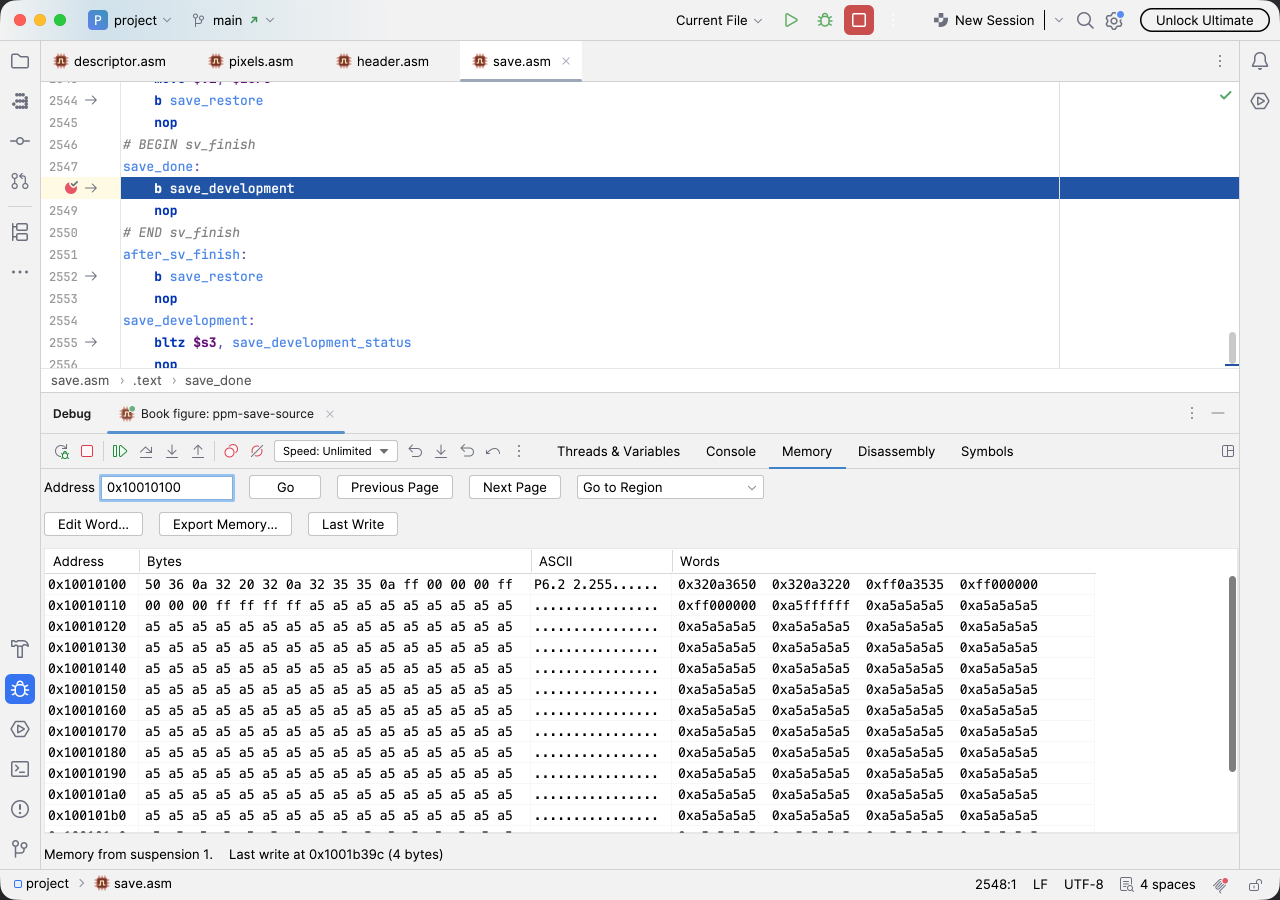
\includegraphics[artifact]{packages/029-binary-ppm/captures/f04/source.png}}
\newsavebox{\MARSppmsaveprivateBox}
\sbox{\MARSppmsaveprivateBox}{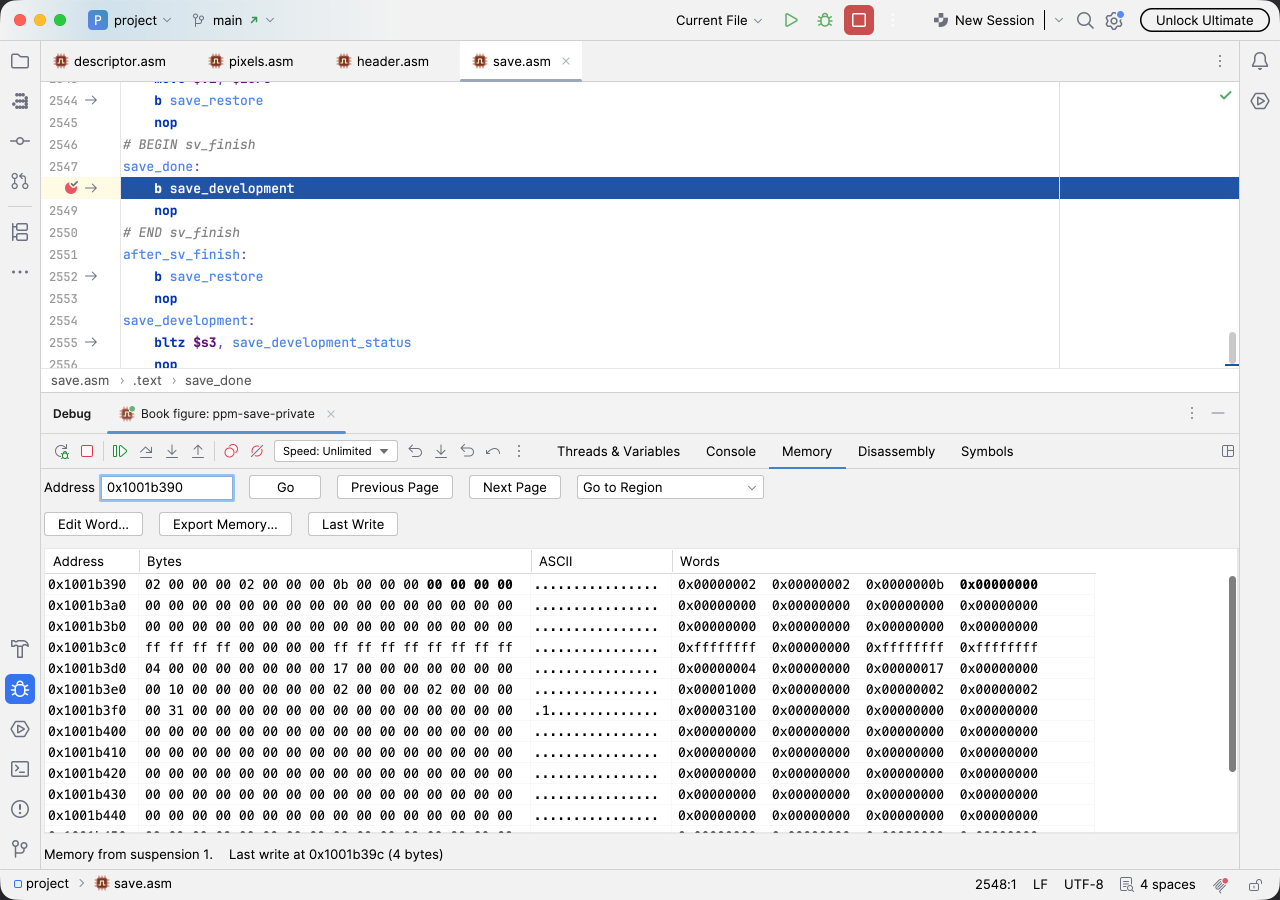
\includegraphics[artifact]{packages/029-binary-ppm/captures/f04/private.png}}
\newsavebox{\MARSppmsavecontrolsBox}
\sbox{\MARSppmsavecontrolsBox}{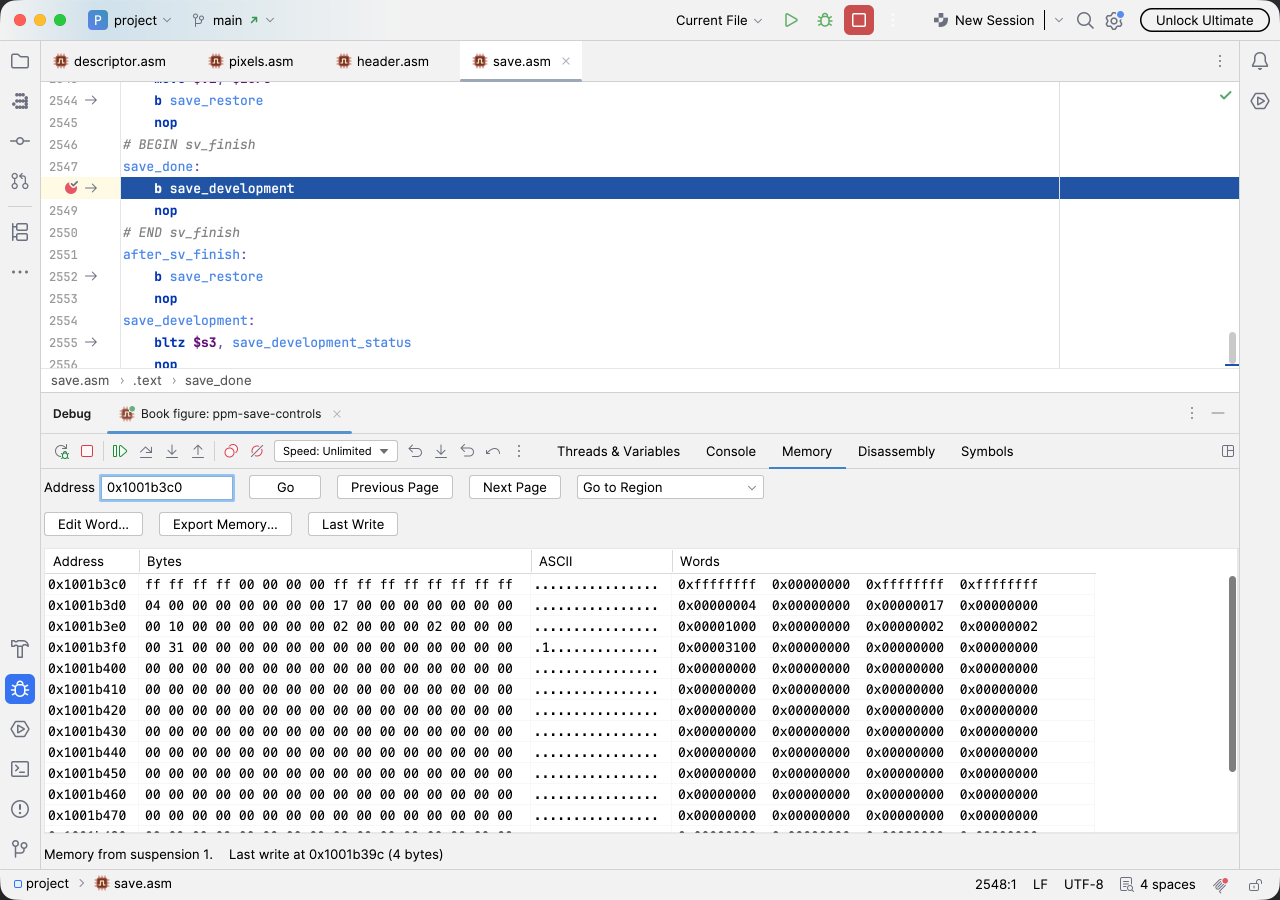
\includegraphics[artifact]{packages/029-binary-ppm/captures/f04/controls.png}}
\edef\MARSppmsavesourceLeft{\the\dimexpr0.036718750\wd\MARSppmsaveregistersBox\relax}
\edef\MARSppmsavesourceBottom{\the\dimexpr0.774444444\ht\MARSppmsaveregistersBox\relax}
\edef\MARSppmsavesourceRight{\the\dimexpr0.713281250\wd\MARSppmsaveregistersBox\relax}
\edef\MARSppmsavesourceTop{\the\dimexpr0.170000000\ht\MARSppmsaveregistersBox\relax}
\edef\MARSppmsaveacceptedLeft{\the\dimexpr0.246093750\wd\MARSppmsaveregistersBox\relax}
\edef\MARSppmsaveacceptedBottom{\the\dimexpr0.077777778\ht\MARSppmsaveregistersBox\relax}
\edef\MARSppmsaveacceptedRight{\the\dimexpr0.553906250\wd\MARSppmsaveregistersBox\relax}
\edef\MARSppmsaveacceptedTop{\the\dimexpr0.874444444\ht\MARSppmsaveregistersBox\relax}
\edef\MARSppmsaveinputLeft{\the\dimexpr0.034375000\wd\MARSppmsavesourceBox\relax}
\edef\MARSppmsaveinputBottom{\the\dimexpr0.311111111\ht\MARSppmsavesourceBox\relax}
\edef\MARSppmsaveinputRight{\the\dimexpr0.584375000\wd\MARSppmsavesourceBox\relax}
\edef\MARSppmsaveinputTop{\the\dimexpr0.608888889\ht\MARSppmsavesourceBox\relax}
\edef\MARSppmsavemetadataLeft{\the\dimexpr0.034375000\wd\MARSppmsaveprivateBox\relax}
\edef\MARSppmsavemetadataBottom{\the\dimexpr0.334444444\ht\MARSppmsaveprivateBox\relax}
\edef\MARSppmsavemetadataRight{\the\dimexpr0.584375000\wd\MARSppmsaveprivateBox\relax}
\edef\MARSppmsavemetadataTop{\the\dimexpr0.608888889\ht\MARSppmsaveprivateBox\relax}
\edef\MARSppmsavecontrolsLeft{\the\dimexpr0.034375000\wd\MARSppmsavecontrolsBox\relax}
\edef\MARSppmsavecontrolsBottom{\the\dimexpr0.311111111\ht\MARSppmsavecontrolsBox\relax}
\edef\MARSppmsavecontrolsRight{\the\dimexpr0.584375000\wd\MARSppmsavecontrolsBox\relax}
\edef\MARSppmsavecontrolsTop{\the\dimexpr0.608888889\ht\MARSppmsavecontrolsBox\relax}
\begin{tikzpicture}[alt={Five details at save_done show native file descriptor three, accepted-byte count twenty-three, the exact source image, private validated metadata and unpublished caller controls. This ordinary host-file capture does not impose the separate core test's three-byte write limit.}]
\node[anchor=north west,inner sep=0,font=\small\bfseries] (source-title) at (6mm,0) {Next unfinished completion region};
\node[anchor=north west,inner sep=0] (source) at ([yshift=-1mm]source-title.south west) {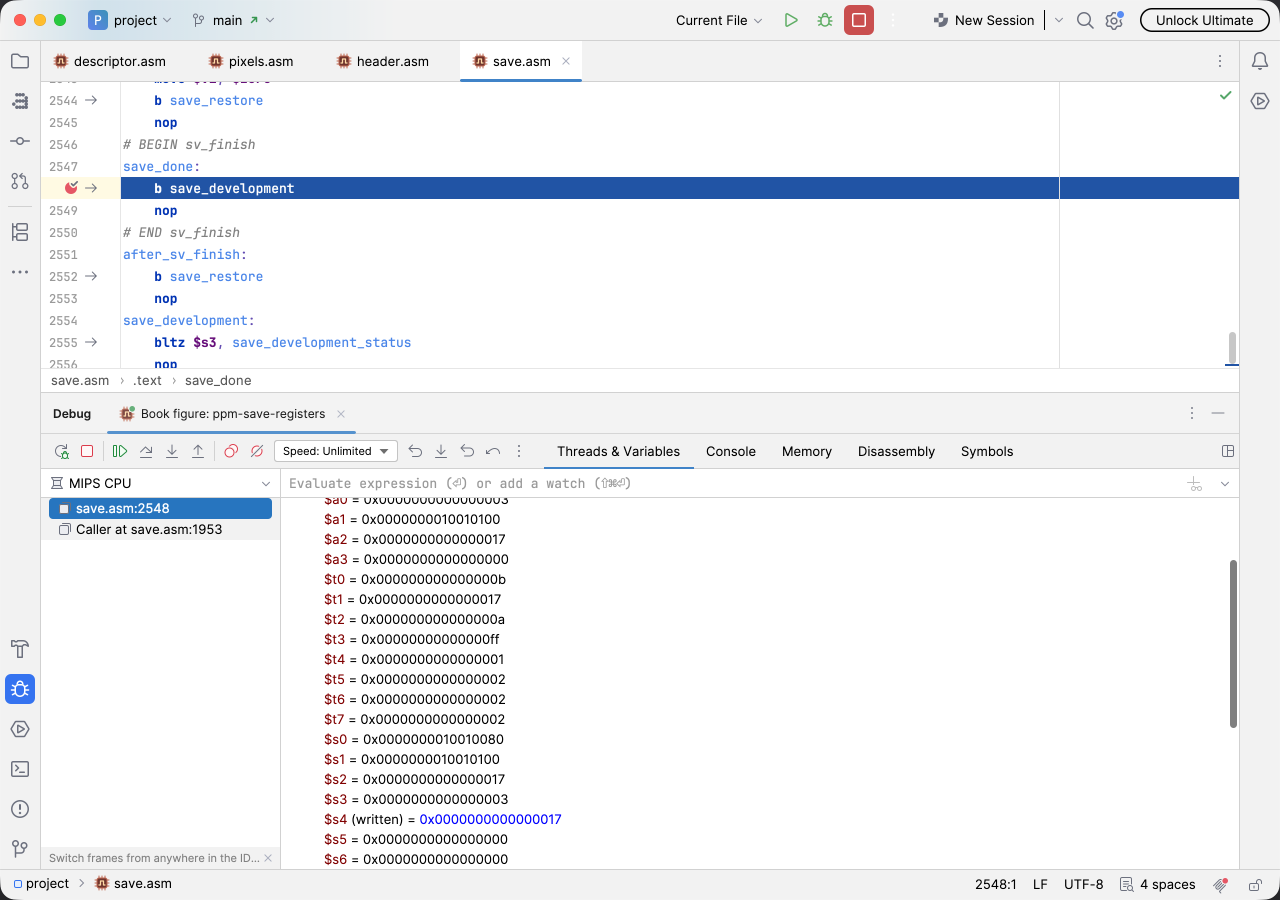
\includegraphics[width=0.54\linewidth,artifact,trim={\MARSppmsavesourceLeft{} \MARSppmsavesourceBottom{} \MARSppmsavesourceRight{} \MARSppmsavesourceTop{}},clip]{packages/029-binary-ppm/captures/f04/registers.png}};
\begin{scope}[shift={(source.south west)},x={($(source.south east)-(source.south west)$)},y={($(source.north west)-(source.south west)$)}]
\draw[black,line width=0.7pt] (0.237500000,0.080000000) rectangle (0.771875000,0.520000000);
\node[draw=black,fill=white,circle,inner sep=1.5pt,font=\footnotesize] at ($(0.237500000,0.520000000)+(-3mm,0)$) {1};
\end{scope}
\node[anchor=north west,inner sep=0,font=\small\bfseries] (accepted-title) at ([yshift=-1mm]source.south west) {Live native descriptor and accepted-byte count};
\node[anchor=north west,inner sep=0] (accepted) at ([yshift=-1mm]accepted-title.south west) {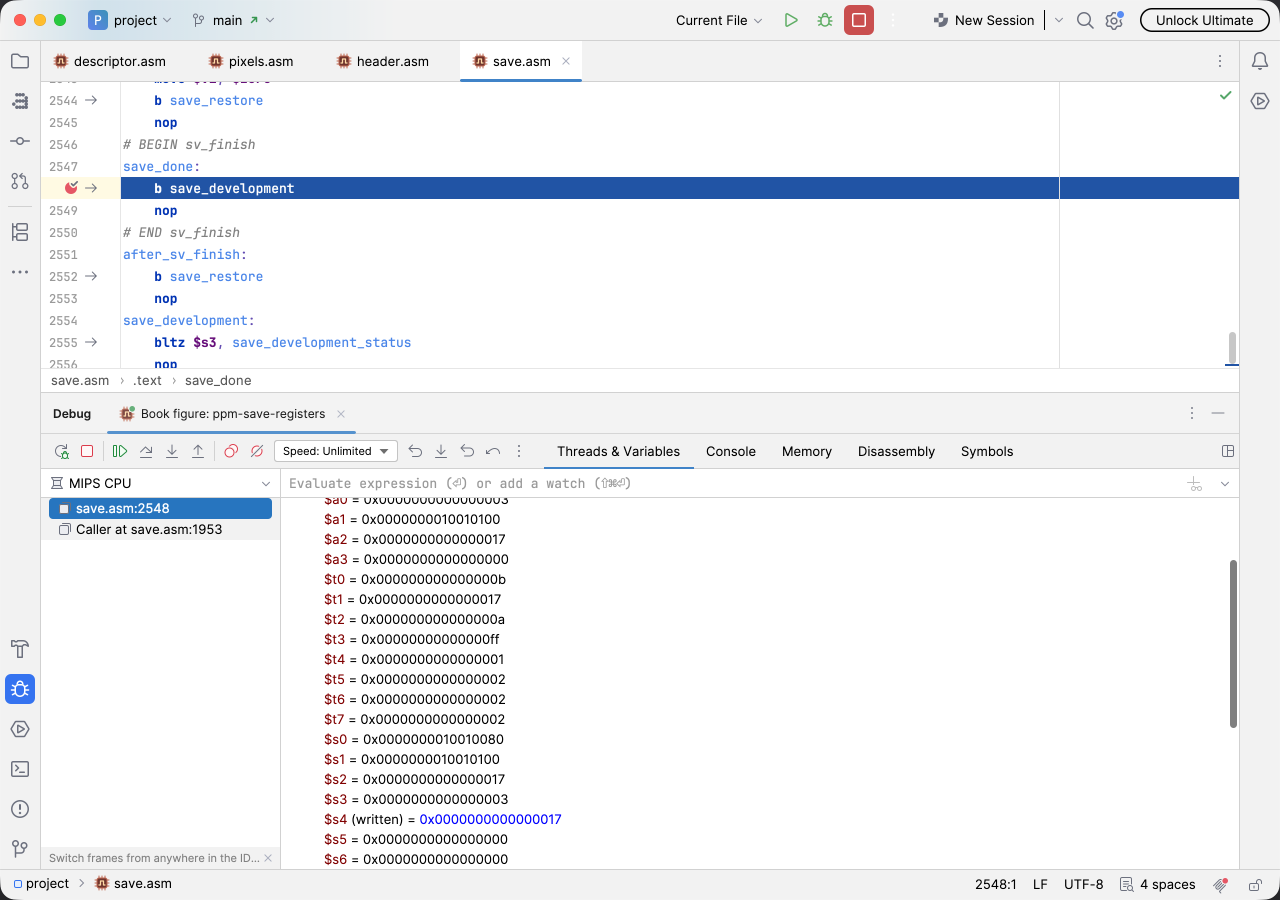
\includegraphics[width=0.52\linewidth,artifact,trim={\MARSppmsaveacceptedLeft{} \MARSppmsaveacceptedBottom{} \MARSppmsaveacceptedRight{} \MARSppmsaveacceptedTop{}},clip]{packages/029-binary-ppm/captures/f04/registers.png}};
\begin{scope}[shift={(accepted.south west)},x={($(accepted.south east)-(accepted.south west)$)},y={($(accepted.north west)-(accepted.south west)$)}]
\draw[black,line width=0.7pt] (0.023437500,0.023255814) rectangle (0.968750000,0.953488372);
\node[draw=black,fill=white,circle,inner sep=1.5pt,font=\footnotesize] at ($(0.023437500,0.953488372)+(-3mm,0)$) {2};
\end{scope}
\node[anchor=north west,inner sep=0,font=\small\bfseries] (input-title) at ([yshift=-1mm]accepted.south west) {Exact twenty-three-byte image};
\node[anchor=north west,inner sep=0] (input) at ([yshift=-1mm]input-title.south west) {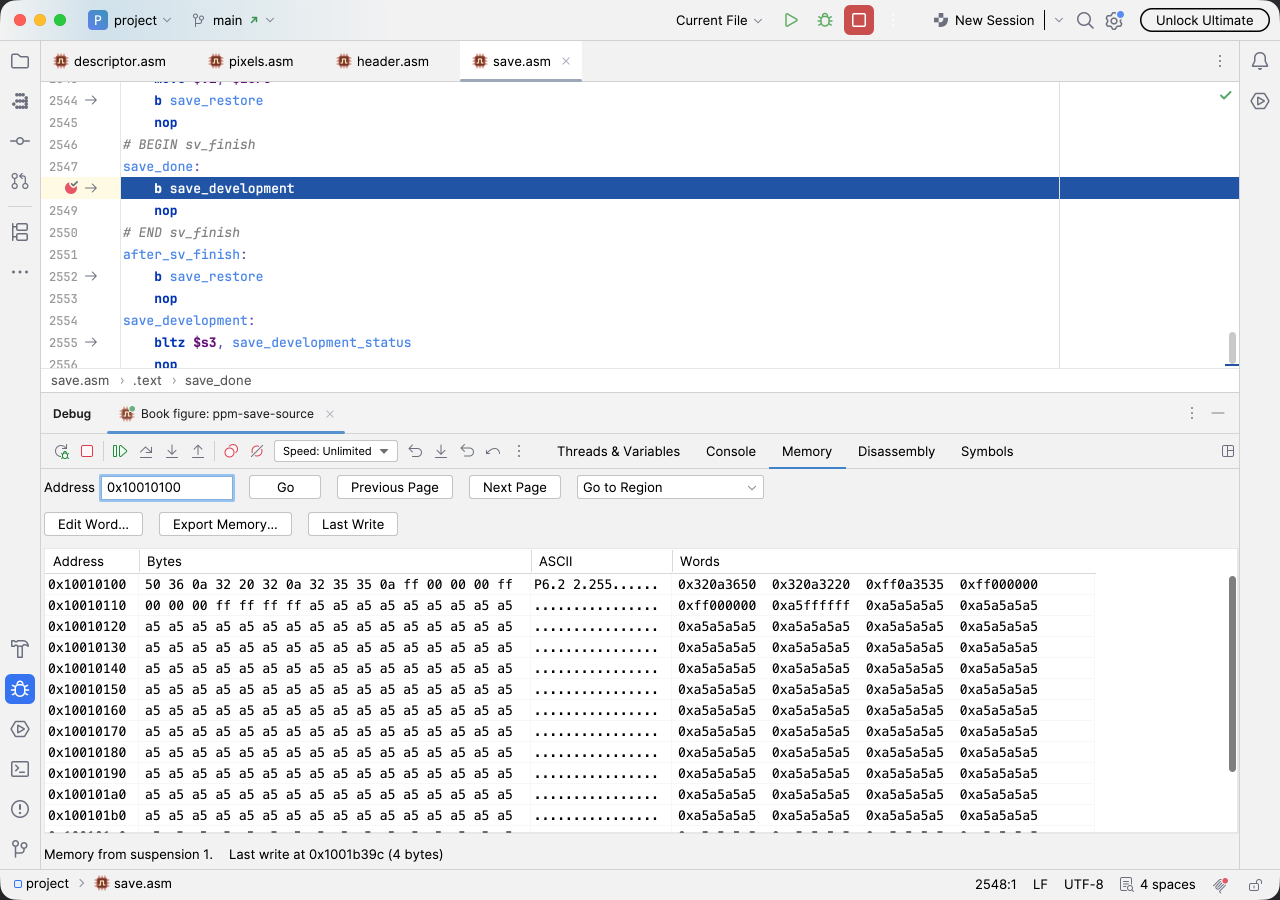
\includegraphics[width=0.84\linewidth,artifact,trim={\MARSppmsaveinputLeft{} \MARSppmsaveinputBottom{} \MARSppmsaveinputRight{} \MARSppmsaveinputTop{}},clip]{packages/029-binary-ppm/captures/f04/source.png}};
\begin{scope}[shift={(input.south west)},x={($(input.south east)-(input.south west)$)},y={($(input.north west)-(input.south west)$)}]
\draw[black,line width=0.7pt] (0.194672131,0.055555556) rectangle (0.997950820,0.638888889);
\node[draw=black,fill=white,circle,inner sep=1.5pt,font=\footnotesize] at ($(0,0.638888889)+(-3mm,0)$) {3};
\end{scope}
\node[anchor=north west,inner sep=0,font=\small\bfseries] (metadata-title) at ([yshift=-1mm]input.south west) {Validation completed before opening output};
\node[anchor=north west,inner sep=0] (metadata) at ([yshift=-1mm]metadata-title.south west) {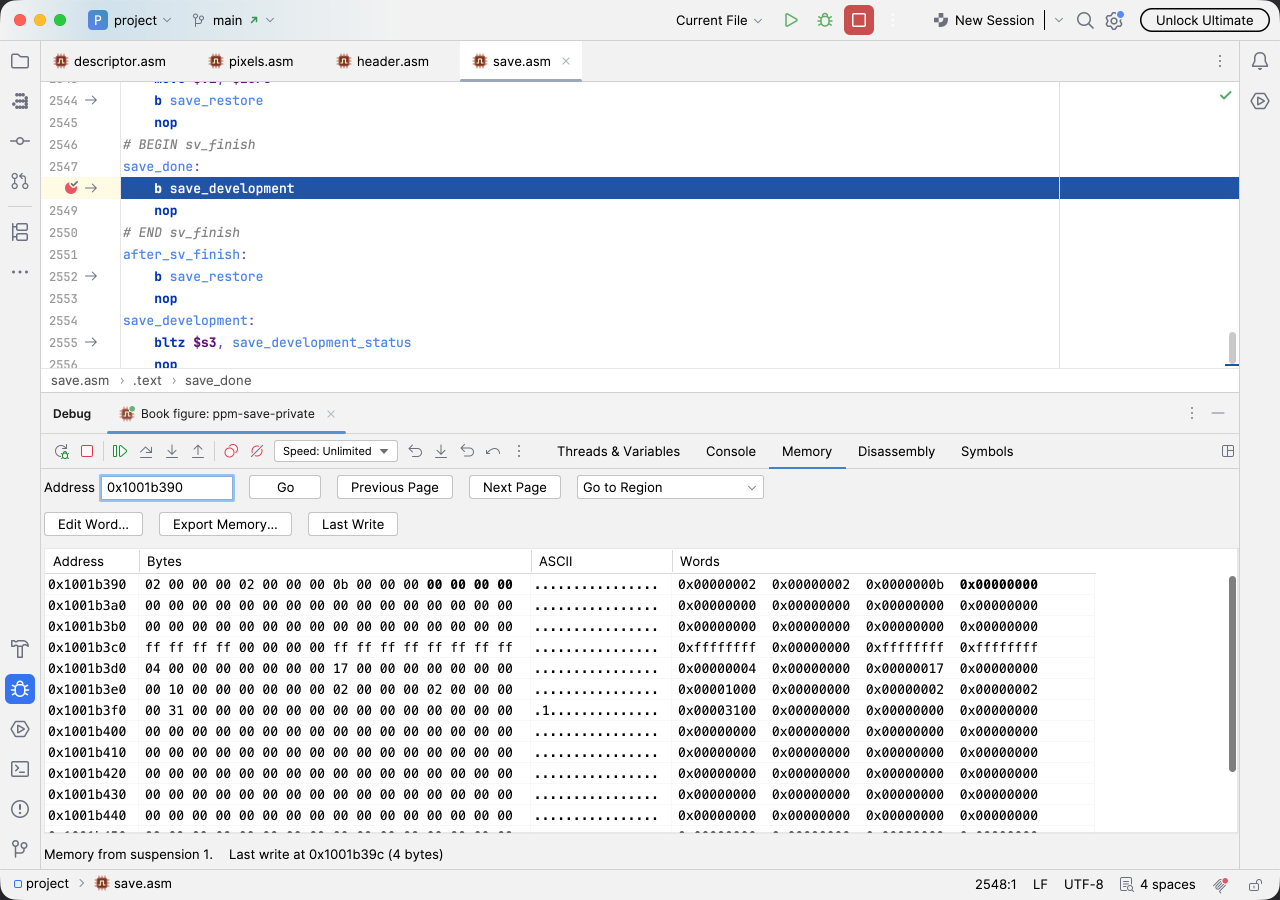
\includegraphics[width=0.84\linewidth,artifact,trim={\MARSppmsavemetadataLeft{} \MARSppmsavemetadataBottom{} \MARSppmsavemetadataRight{} \MARSppmsavemetadataTop{}},clip]{packages/029-binary-ppm/captures/f04/private.png}};
\begin{scope}[shift={(metadata.south west)},x={($(metadata.south east)-(metadata.south west)$)},y={($(metadata.north west)-(metadata.south west)$)}]
\draw[black,line width=0.7pt] (0.194672131,0.078431373) rectangle (0.997950820,0.490196078);
\node[draw=black,fill=white,circle,inner sep=1.5pt,font=\footnotesize] at ($(0,0.490196078)+(-3mm,0)$) {4};
\end{scope}
\node[anchor=north west,inner sep=0,font=\small\bfseries] (controls-title) at ([yshift=-1mm]metadata.south west) {Caller results remain unpublished};
\node[anchor=north west,inner sep=0] (controls) at ([yshift=-1mm]controls-title.south west) {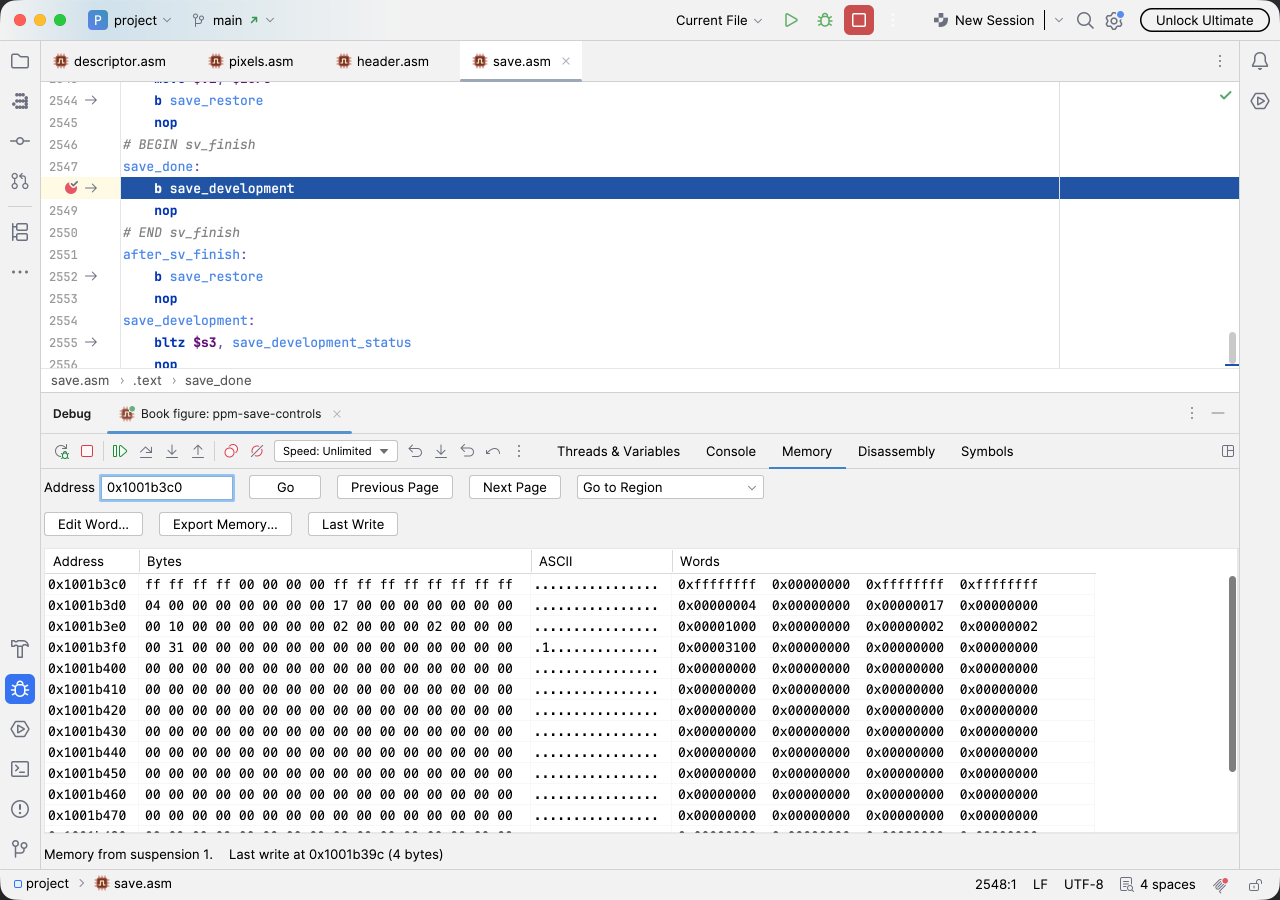
\includegraphics[width=0.84\linewidth,artifact,trim={\MARSppmsavecontrolsLeft{} \MARSppmsavecontrolsBottom{} \MARSppmsavecontrolsRight{} \MARSppmsavecontrolsTop{}},clip]{packages/029-binary-ppm/captures/f04/controls.png}};
\begin{scope}[shift={(controls.south west)},x={($(controls.south east)-(controls.south west)$)},y={($(controls.north west)-(controls.south west)$)}]
\draw[black,line width=0.7pt] (0.194672131,0.055555556) rectangle (0.997950820,0.638888889);
\node[draw=black,fill=white,circle,inner sep=1.5pt,font=\footnotesize] at ($(0,0.638888889)+(-3mm,0)$) {5};
\end{scope}
\end{tikzpicture}
\par\smallskip
\begin{minipage}{\linewidth}
\small
\begin{enumerate}
\setlength{\itemsep}{0pt}
\setlength{\parsep}{0pt}
\item At \texttt{save\_done}, the write loop has accepted all bytes. The highlighted branch belongs to the unfinished \texttt{sv\_finish} region. The final success selection and normal completion code are the next lesson\textquotesingle s edit.
\item \texttt{s3 = 3} is the descriptor returned by this native IDE run. \texttt{s4 = 0x17}, decimal twenty-three, is the accumulated accepted-byte count. The routine retains its descriptor across writes and advances by the syscall\textquotesingle s actual result. A descriptor identifies an open file; it is not a byte count.
\item The source contains the eleven-byte header and twelve raster bytes. Only those twenty-three logical bytes are written. The displayed \texttt{a5} suffix is backing storage, not additional file content.
\item The private descriptor records the validation result: width two, height two and offset eleven. Validation precedes opening the output, so malformed input can be rejected without truncating an existing file.
\item The caller\textquotesingle s saved status and count are still $-1$. These photographs use ordinary host-file writes and native descriptor three. The separate core recipe forces three-byte writes and descriptor nine. Both reach accepted count twenty-three; this unfinished stage then closes its owned descriptor and returns development status four with count zero.
\end{enumerate}
\end{minipage}
\caption{Accepted file bytes precede the routine completion and descriptor close.}
\label{capture:029-binary-ppm-f04}
\label{ppm-f04}
\end{figure}
\par
